\documentclass{beamer}
\usepackage{minted}
\usepackage{graphicx}
\usepackage[utf8]{inputenc}
\setbeamertemplate{navigation symbols}{}

\title{\LaTeX}

\subtitle{lay-teck}

\author{Some Guy}
\institute{Linux@APP}
\date{02/21/2018}
 
\begin{document}

\frame{\titlepage}

\begin{frame}[fragile]
\frametitle{A frame}
Framy stuff.

{\LaTeX} or \verb|\LaTeX|
\begin{verbatim}
\documentclass{beamer}
\title{\LaTeX}
\subtitle{lay-teck}
\author{Some Guy}
\institute{Linux@APP}
\date{02/21/2018}

\begin{document}

\frame{\titlepage}


\end{verbatim}


\end{frame}

% Python3 code
\begin{frame}[fragile]

% must install pygments for minted to work can be 2 or 3
% run latex compiler with -shell-escape as well
\begin{minted}{python3}

#Leibniz formula

pi = 0
x = 0
iterations = 10000
try:
        for x in range(iterations):
                pi = pi + 2 / ((4*x+1) * (4*x+3))
        print(pi*4)

except KeyboardInterrupt:
        print(x)
        print(pi*4)


\end{minted}

\end{frame}

\begin{frame}
tlmgr update --list

tlmgr update --self

tlmgr update --all

tlmgr uninstall
\begin{figure}{Fig. 1: I got this off of reddit.}
\centering
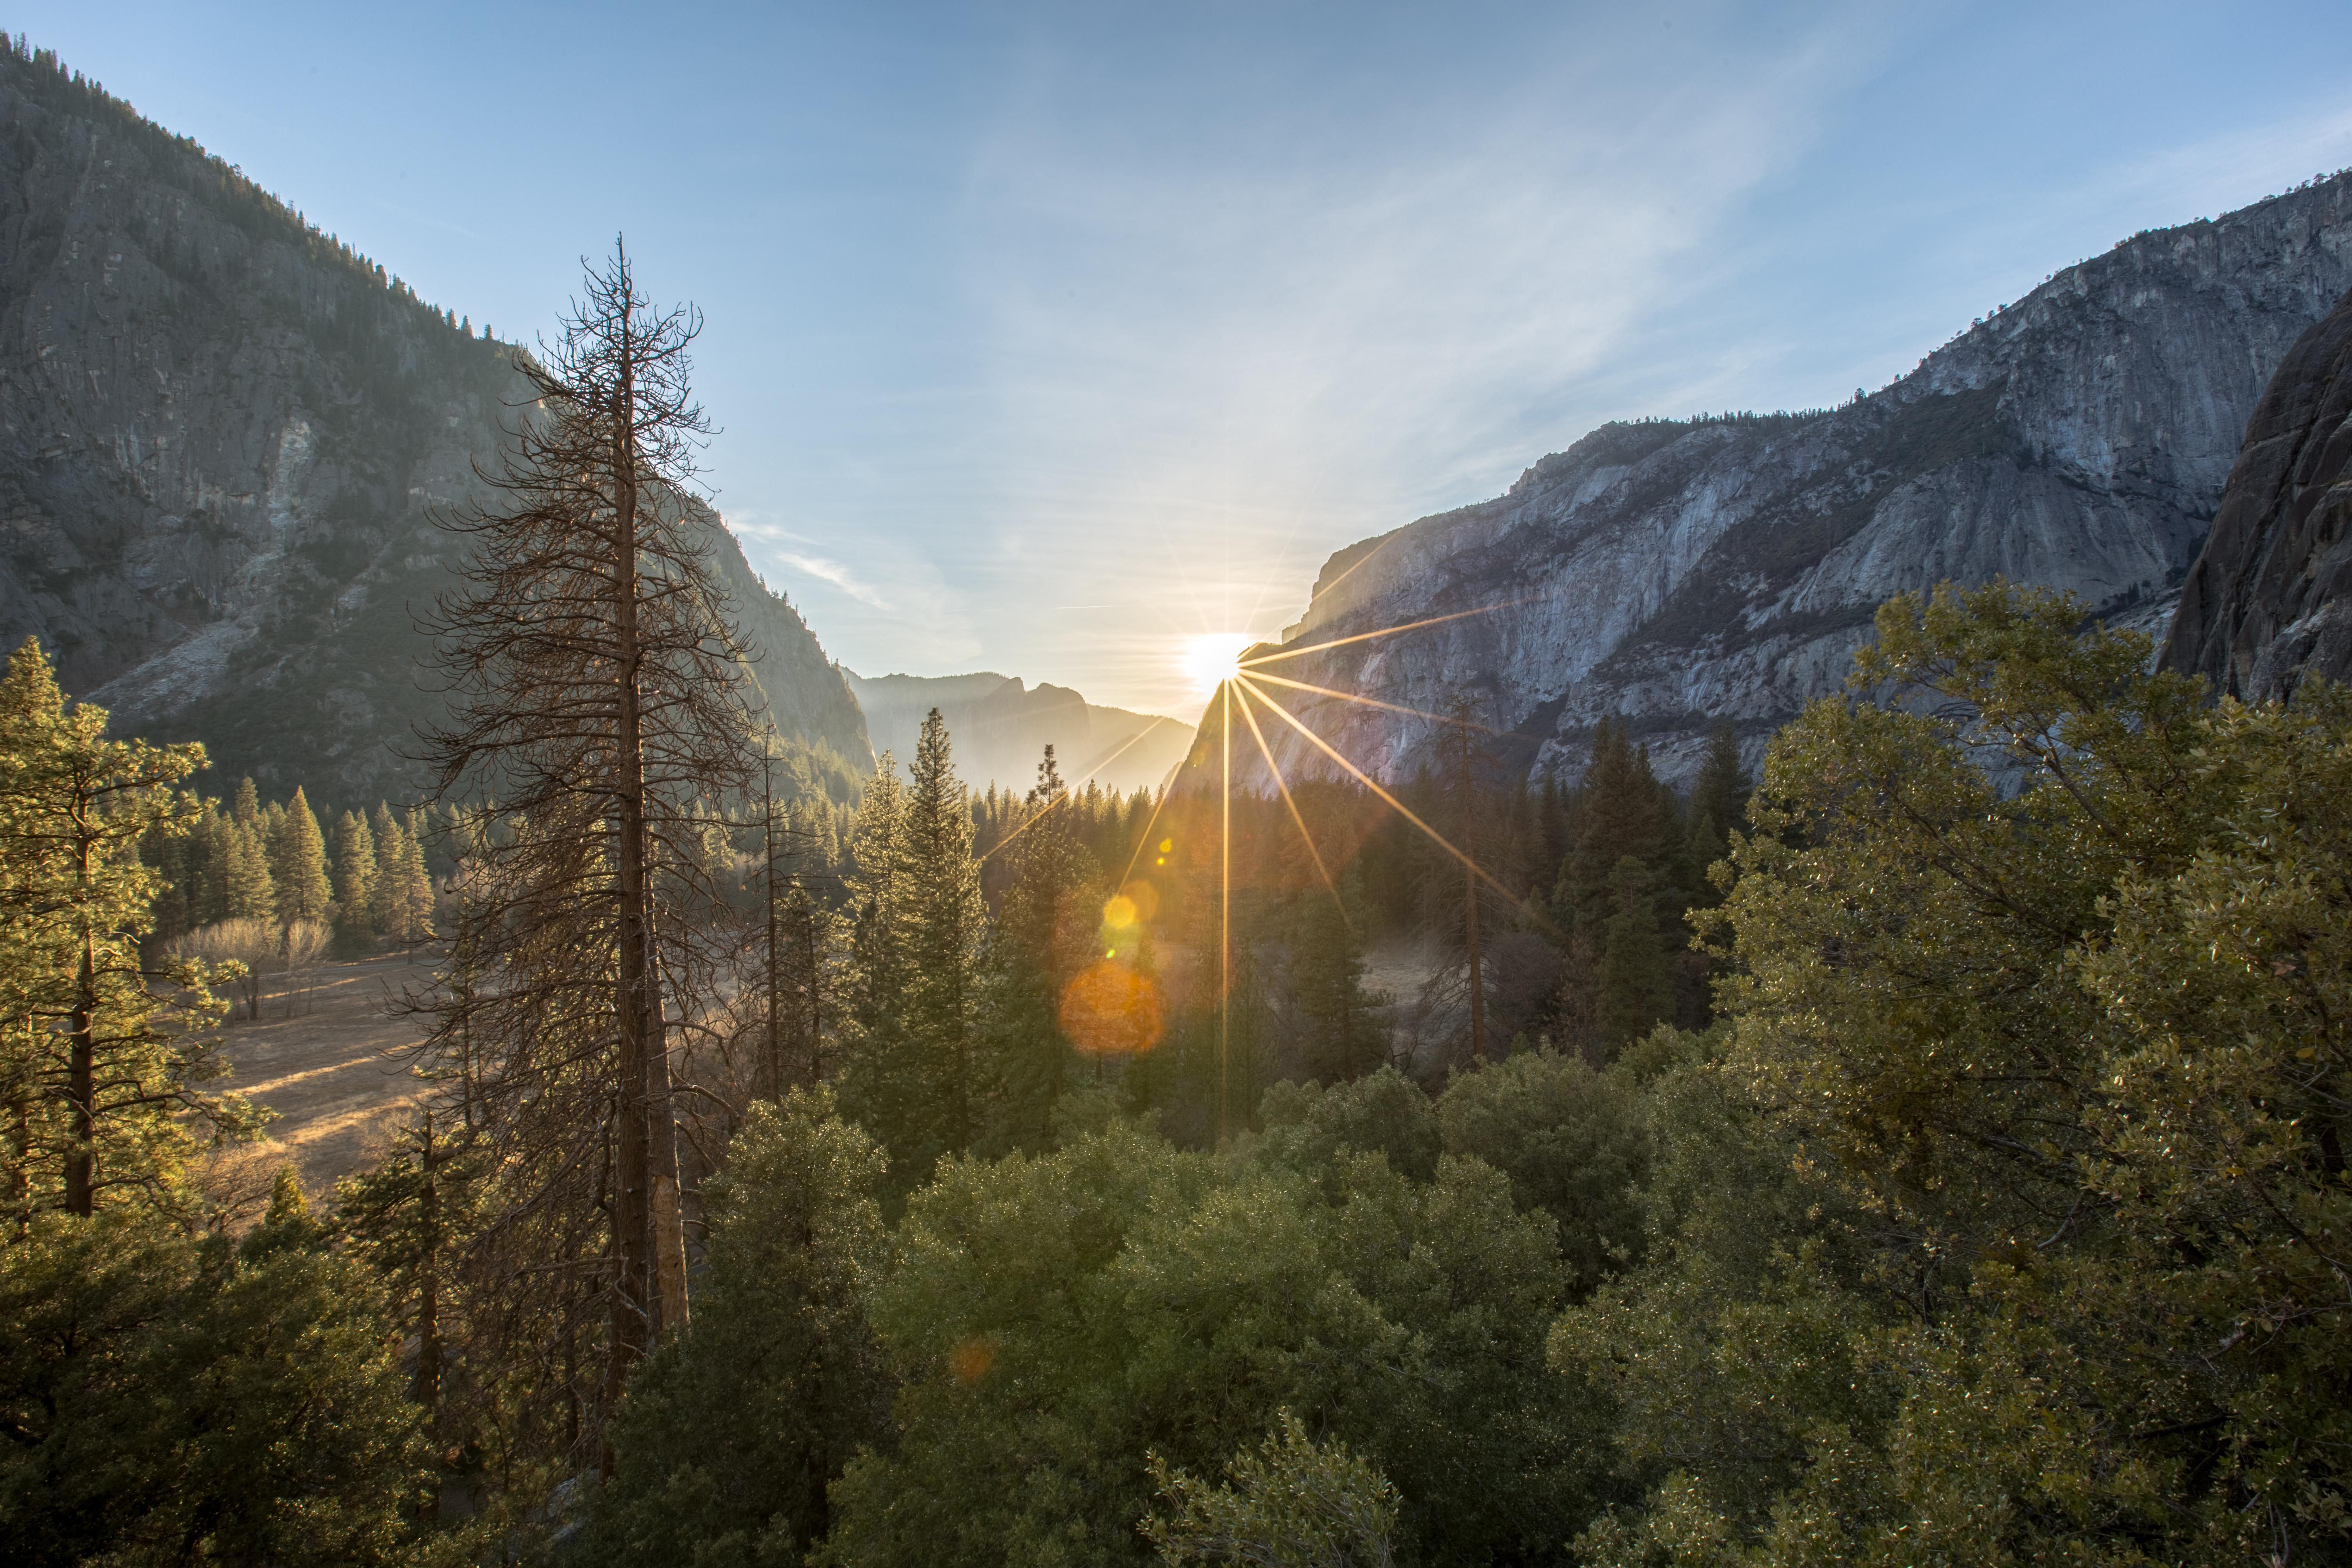
\includegraphics[height=2.5in]{picture1}
\end{figure}
\end{frame}

% bash stuff
\begin{frame}[fragile]
% must install pygments for minted to work can be 2 or 3
% run latex compiler with -shell-escape as well
\input{cowsay}
\end{frame}

\begin{frame}[fragile]
\begin{minted}{latex}
\LaTeX
\end{minted}
\end{frame}

\end{document}
